\documentclass{svproc}

\usepackage{url}
\usepackage{amsmath}
\usepackage{amssymb}
\usepackage{soul}
\usepackage{graphicx}
\usepackage{seqsplit}
\usepackage{tikz}
\usepackage[ruled,vlined,linesnumbered]{algorithm2e}
\usepackage[colorlinks=true, linkcolor=blue, citecolor=blue, urlcolor=blue]{hyperref}

\SetKwProg{Let}{let}{be:}{}
\usetikzlibrary{arrows, decorations.pathmorphing, decorations.markings, shapes.geometric, calc, positioning}

\tikzset{
    node0/.style={circle, draw, fill=white, inner sep=0pt, minimum size=1.5mm},
    node1/.style={circle, draw, fill=black, inner sep=0pt, minimum size=1.5mm},
    reoEdge/.style={->, >=latex, thin},
    reoSpout/.style={<->, >=latex, thin},
    reoLossy/.style={->, >=latex, thin, dashed},
    reoWavy/.style={->, >=latex, thin, decorate, decoration={zigzag, amplitude=1mm, segment length=1.5mm, post length=1.5mm, pre length=1.5mm}},
}

% A. 基础连线类 (Sync, Lossy, Filter)  参数: #1=样式(可选), #2=起点, #3=终点, #4=标签文字(可选)
\newcommand{\drawLink}[4][reoEdge]{
    \draw[#1] (#2) -- node[above, font=\scriptsize] {#4} (#3);
}

% B. FIFO 类 (中间带方框)  参数: #1=起点, #2=终点, #3=方框内文字, #4=额外样式(可选,如 dashed)
\newcommand{\drawFIFO}[4][]{
    \draw[reoEdge, #1] (#2) -- node[midway, sloped, allow upside down, draw, fill=white, rectangle, minimum width = 6mm, minimum height = 2mm, inner sep=1pt, font=\tiny] {#4} (#3);
}

% C. Drain 类 (两头向中间汇聚)  参数: #1=起点1, #2=起点2, #3=汇聚点/符号位置(通常是这两个点的中点), #4=中心符号(如 ||)
\newcommand{\drawDrain}[5]{
    % 计算中点
    \coordinate (mid1) at ($(#1)!0.4!(#2)$);
    \coordinate (mid) at ($(#1)!0.5!(#2)$);
    \coordinate (mid2) at ($(#1)!0.6!(#2)$);
    % 画两段箭头指向中点
    \draw[->, >=latex, thin] (#1) -- (mid1);
    \draw[thin] (mid1) -- (mid);
    \draw[thin] (mid) -- (mid2);
    \draw[->, >=latex, thin] (#2) -- (mid2);
    % 画中心符号
    \node at (mid) [font=\tiny, inner sep=1pt] {#3};
    \node at (mid1) [font=\tiny, inner sep=1pt] {#4};
    \node at (mid2) [font=\tiny, inner sep=1pt] {#5};
    % 实际上 Drain 并没有显式的 Sink 节点,这里 #3 只是为了兼容位置逻辑,或者如果不画节点只画线
}

% D. Spout 类 (一点分发给两点)  参数: #1=源点, #2=终点1, #3=终点2, #4=线样式
\newcommand{\drawSpout}[5]{
    % 计算中点
    \coordinate (mid1) at ($(#1)!0.4!(#2)$);
    \coordinate (mid) at ($(#1)!0.5!(#2)$);
    \coordinate (mid2) at ($(#1)!0.6!(#2)$);
    % 画两段箭头指向中点
    \draw[->, >=latex, thin] (mid1) -- (#1);
    \draw[thin] (mid1) -- (mid);
    \draw[thin] (mid) -- (mid2);
    \draw[->, >=latex, thin] (mid2) -- (#2);
    % 画中心符号
    \node at (mid) [font=\tiny, inner sep=1pt] {#3};
    \node at (mid1) [font=\tiny, inner sep=1pt] {#4};
    \node at (mid2) [font=\tiny, inner sep=1pt] {#5};
    % 实际上 Drain 并没有显式的 Sink 节点,这里 #3 只是为了兼容位置逻辑,或者如果不画节点只画线
}

% E. Timer 类 (中间带圆角框)  参数: #1=起点, #2=终点, #3=延迟时间 t
\newcommand{\drawTimer}[3]{
    \draw[reoEdge] (#1) -- node[draw, fill=white, rectangle, rounded corners=2pt, minimum size=3.5mm, inner sep=1pt, font=\tiny] (timerbox) {#3} (#2);
}

% F. 复杂 Timer 类 (带控制端口 OFF/RESET/EXPIRE)  参数: #1=起点, #2=终点, #3=延迟时间 t, #4=控制类型(OFF/RST/EXP), #5=控制节点位置(above/below)
\newcommand{\drawComplexTimer}[5]{
    % 先画基础 Timer
    \draw[reoEdge] (#1) -- node[draw, fill=white, rectangle, rounded corners=2pt, minimum size=3.5mm, inner sep=1pt, font=\tiny] (timerbox) {#3} (#2);
    % 画控制端口
    \node (ctrl) [#5=0.5cm of timerbox, font=\tiny] {#4};
    \draw[->, >=latex, dashed] (ctrl) -- (timerbox);
}


% --- 1. Basic Channels ---
\newcommand{\chanSync}[2]{\drawLink{#1}{#2}{}}
\newcommand{\chanLossySync}[2]{\drawLink[reoLossy]{#1}{#2}{}}
\newcommand{\chanSyncDrain}[2]{\drawDrain{#1}{#2}{}{}{}} % 空心汇聚
\newcommand{\chanAsynDrain}[2]{\drawDrain{#1}{#2}{$||$}{}{}} % 带竖线汇聚
% --- 2. FIFO Variants ---
\newcommand{\chanFifoOne}[2]{\drawFIFO{#1}{#2}{}}          % Buffer size 1
\newcommand{\chanFifoN}[3]{\drawFIFO{#1}{#2}{$N=#3$}}      % Buffer size n
\newcommand{\chanFifoOneE}[3]{\drawFIFO{#1}{#2}{$#3$}}     % Initialized with e
\newcommand{\chanFifoNE}[4]{\drawFIFO{#1}{#2}{$#3$}}    % Initialized e with size n
% --- 3. Filter & Producer ---
\newcommand{\chanFilterP}[3]{\drawLink[reoWavy]{#1}{#2}{$P(#3)$}} 
\newcommand{\chanProducerP}[3]{\drawLink{#1}{#2}{Prod: $#3$}} 
% --- 4. Spouts ---
\newcommand{\chanSyncSpout}[2]{\drawSpout{#1}{#2}{}{}{}}
\newcommand{\chanAsynSpout}[2]{\drawSpout{#1}{#2}{$||$}{}{}}
% --- 5. Probabilistic/Faulty ---
\newcommand{\chanCptSync}[3]{\drawLink{#1}{#2}{$p=#3$}}       % Corrupting Sync
\newcommand{\chanRdmSync}[3]{\drawLink{#1}{#2}{#3}}         % Random Sync
\newcommand{\chanProbLossy}[3]{\drawLink[reoLossy]{#1}{#2}{$p=#3$}} % Probabilistic Lossy
\newcommand{\chanFtyFifoOne}[3]{\drawFIFO{#1}{#2}{Fty:$#3$}} % Faulty FIFO
\newcommand{\chanLossyFifoOne}[3]{\drawFIFO[dashed]{#1}{#2}{Lossy:$#3$}} % Lossy FIFO
% --- 6. Timers ---
\newcommand{\chanTimert}[3]{\drawTimer{#1}{#2}{#3}}
\newcommand{\chanOFFTimert}[3]{\drawComplexTimer{#1}{#2}{#3}{OFF}{above}}
\newcommand{\chanRSTTimert}[3]{\drawComplexTimer{#1}{#2}{#3}{RST}{above}}
\newcommand{\chanEXPTimert}[3]{\drawComplexTimer{#1}{#2}{#3}{EXP}{above}}

\bibliographystyle{splncs03}
\def\UrlFont{\rmfamily}

\begin{document}

\title{Connectors as designs: Refinement and test case generation using Z3}
\titlerunning{Connectors as designs: Refinement and test case generation using Z3}
\author{Sihan Wu\inst{1} \and Xueyi Tan\inst{2}}
\authorrunning{S. Wu and X. Tan}
\tocauthor{Wu, Tan}
\institute{Yuanpei College, Peking University, No.5 Yiheyuan Road, Haidian District, Beijing 100871, China,\\
\email{2300017743@stu.pku.edu.cn},
\and
School of Mathematical Sciences, Peking University, No.5 Yiheyuan Road, Haidian District, Beijing 100871, China,\\
\email{2300010816@stu.pku.edu.cn}}

\maketitle

\begin{abstract}
test. test.
\keywords{test, test, test}
\end{abstract}
\section{Introduction}


\section{Preliminaries}
\subsection{The coordination language Reo}
Reo is a channel-based exogenous coordination language where complex coordinators, called connectors, are compositionally built out of simpler ones \cite{Reo}. Exogenous coordination imposes a purely local interpretation on each inter-component communication, engaged in as a pure I/O operation on each side, that allows components to communicate anonymously, through the exchange of untargeted passive data.\par
Complex connectors in Reo are organized in a network of primitive connectors with well-defined behavior, called \textit{channels}, such as synchronous channels, FIFO channels, etc. A connector provides the protocol that controls and organized the communication, synchronization and cooperation among the components/services that they interconnect. Each channel has two \textit{channel ends}: \textit{source} ends and \textit{sink} ends. A source channel end accepts data into the channel, and a sink channel end dispenses data out of the channel. It is possible for the ends of a channel to be both sinks or both sources. Reo places no restriction on the behavior of a channel and thus allows an open-ended set of different channel types to be used simultaneously together. Each channel end can be connected to at most one component instance at any given time. Some simple channel types in Reo are shown in section{Modeling Connectors}.\par
Complex connectors are constructed by composing simpler ones via the \textit{join} and \textit{hiding} operations. Channels are joined together at nodes. A node consists of a set of channel ends. The set of channel ends coincident on a node $A$ is disjointly partitioned into the sets Src($A$) and Snk($A$), denoting the sets of source and sink channel ends that coincide on $A$, respectively. Nodes are categorized into \textit{source}, \textit{sink} and \textit{mixed nodes}, depending on whether all channel ends that coincide on a node are source ends, sink ends or a combination of the two. The hiding operation is used to hide the internal topology of a component connector. The hidden nodes can no longer be accessed or observed from outside. A complex connector has a graphical representation, called a \textit{Reo circuit}, which is a finite graph where the nodes are labeled with pair-wise disjoint, non-empty sets of channel ends, and the edges represent their connecting channels. The behavior of a Reo circuit is formalized by means of the data-flow at its sink and source nodes. Intuitively, the source nodes of a circuit are analogous to the input ports, and the sink nodes to the output ports of a component, while mixed nodes capture its hidden internal details.\par
A component can write data items to a source node that it is connected to. The write operation succeeds only if all (source) channel ends coincident on the node accept the data item, in which case the data item is transparently written to every source end coincident on the node. A source node, thus, acts as a replicator. A component can obtain data items, by an input operation, from a sink node that it is connected to. A take operation succeeds only if at least one of the (sink) channel ends coincident on the node offers a suitable data item; if more than one coincident channel end offers suitable data items, one is selected non-deterministically. A sink node, thus, acts as a non-deterministic merger. A mixed node nondeterministically selects and takes a suitable data item offered by one of its coincident sink channel ends and replicates it into all of its coincident source channel ends. Note that a component cannot connect to, take from, or write to mixed nodes.

\subsection{The UTP observational model}
Specification and unification phases can be observed in every scientific discipline. During specification sicentists focus on some narrowly defined phenomenon and aim to discover the laws governing that phenomenon, which, typically, are special cases of a more general theory. Unification aims at unifying theory that clearly and convincingly exlains a broader range of phenomena. A proposed unification of theories often receives spectacular confirmation and reward complementary to the prediction of new discoveries or by the development of new technologies. However, a unifying theory is usually complementary to the theories that it links, and does not seek to replace them. In \cite{hoare1997unified} Hoare and He aim at unification in computer science. They saw the need for a comprehensive theory of programming that
\begin{itemize}
    \item includes a convincing approach to the study of a range of languages in which computer programs may be expressed,
    \item must introduce basic concepts and properties that are common to the whole range of programming methods and languages,
    \item must deal separately with the additions and variations that are particular to specific groups of related languages,
    \item should aim to treat each aspect and feature in the simplest possible fashion and in isolation from all the other features with which it may be combined or confused.
\end{itemize}
Our theory of Reo connectors originated out of these motivations for unification. In this section we introduce the theory of UTP designs and the observational model for connectors briefly. More details about UTP can be found in \cite{hoare1997unified}.

\subsubsection{A theory of designs}
UTP adopts the relational calculus as the foundation to unify various programming theories. All kinds of specifications, designs and programs are interpreted as relations between an initial observation and a subsequent (intermediate, stable or final) observation of the behavior of their execution. Program correctness and refinement can be represented by inclusion of relations, and all laws of the relational calculus are valid for reasoning about correctness.\par
Collections of relations form a theory of the paradigm being studied, and it contains three essential parts: an alphabet, a signature, and healthiness conditions.\par
During observations it is usual to wait for some initial transient behavior to stabilize before making any further observation. In order to express this, we introduce two varaibles \textit{ok}, \textit{ok'}: \textbf{Boolean}. The variable \textit{ok} stands for a successful initialization and the start of a communication. When \textit{ok} is \textbf{false}, the communication has not started, so no observation can be made. The variable \textit{ok'} denotes the observation that the communication has either terminated or reached an intermediate stable state. The communication is divergent when \textit{ok'} is \textbf{false}.\par
In our semantic model, the observational semantics for a Reo connector is described by a design, i.e., a relation expressed as $P\vdash Q$, where $P$ is the predicate specifying the relationship among the observations on the source nodes of the connector, and $Q$ is the predicate specifying the condition that should be satisfied by the observations on the sink nodes of the connector. Such a design $P\vdash Q$ is defined as follows:
\begin{definition}
    A design is a pair of predicates $P\vdash Q$, where neither predicate contains \textit{ok} or \textit{ok'}, and $P$ has only unprimed variables. It has the following meaning:$$P\vdash Q=_{df}(ok\land P\Rightarrow ok'\land Q)$$
    \label{def:1}
\end{definition}
A design predicate represents a pre/post-condition specification. The separation of precondition from post-condition allows us to write a specification that has a more general precondition than simply the domain of the relation used as a specification. Implementing a design, we are allowed to assume that the precondition holds, but we have to satisfy the post-condition. Moreover, we can rely on the system having been started, but we must ensure that it terminates. If the precondition does not hold, or the system does not start, we are not committed to establish the post-condition nor even to make the system terminate.
Any non-trivial system requires a facility to select between alternatives according to the truth or falsehood of some guard condition $b$. The restriction that b contains no primed variables ensures that it can be checked before starting either of the actions. The conditional expression $P\triangleleft b\triangleright Q$ describes a system that behaves like $P$ if the initial value of $b$ is \textbf{true}, or like $Q$ otherwise. It can be defined as follows:
\begin{definition}
    The conditional expression is defined as follows:$$P\triangleleft b\triangleright Q=_{df}(\textbf{true}\vdash(b\land P\lor \lnot b\land Q))$$
\end{definition}
The sequential composition $P$; $Q$ denotes a system that first executes $P$, and when $P$ terminates executes $Q$. This system is defined via existential quantification to hide its intermediate observation, and to remove the variables that record this observation from the list of free variables of the predicate. To accomplish this hiding, we introduce a fresh set of variables $v_0$ to denote the intermediate observation. These fresh variables replace the input variables $v$ of $Q$ and the output variables $v'$ of $P$, thus the output alphabet of $P$ ($out_{\alpha}P$) and the input alphabet of $Q$ ($in_{\alpha}Q$) must be the same.
\begin{definition}
    Let $out_{\alpha}P=\{v'\}$, $in_{\alpha}Q=\{v\}$, then
    $$P(in:u;out:v');Q(in:v;out:w)=_{df}\exists v_0\cdot P(in:u;out:v_0)\land Q(in:v;out:w)$$
\end{definition}
If the conditional and sequential operators are applied to designs, the result is also a design. This follows from the laws below.
\[
\begin{split}
    &(P_1\vdash Q_1)\triangleleft b\triangleright(P_2\vdash Q_2)=((P_1\triangleleft b\triangleright P_2)\vdash(Q_1\triangleleft b\triangleright Q_2))\\
    &(P_1\vdash Q_1);(P_2\vdash Q_2)=(P_1\land\lnot(Q_1;\lnot P_2)\vdash(Q_1;Q_2))
\end{split}
\]
A reassuring result about a design is the notion of refinement, which is defined via implication. In UTP, we have the well-known property that under refinement, preconditions are weakened and post-conditions are strengthened. This is established by the following definition:
\begin{definition}
    $[(P_1\vdash Q_1)\sqsubseteq(P_2\vdash Q_2)]$ \textbf{iff} $[P_1\Rightarrow P_2]\land[P_1\land Q_2\Rightarrow Q_1]$
\end{definition}
The theory of designs forms a complete lattice, with miracle $\top_{\textbf{D}}$ as the top element, and abort $\bot_{\textbf{D}}$ as the bottom element.
$$\top_{\textbf{D}}=_{df}(\textbf{true}\vdash\textbf{false})\text{ and }\bot_{\textbf{D}}=_{df}(\textbf{false}\vdash\textbf{true})$$
The meet and join operations in the lattice of designs are defined as follows, which represent internal (non-deterministic, demonic) and external (angelic) choices.
\[
\begin{split}
    (P_1\vdash Q_1)\sqcap(P_2\vdash Q_2)&=(P_1\land P_2\vdash Q_1\lor Q_2)\\
    (P_1\vdash Q_1)\sqcup(P_2\vdash Q_2)&=(P_1\lor P_2\vdash ((P_1\Rightarrow Q_1)\land(P_2\Rightarrow Q_2)))
\end{split}
\]
Finally, iteration is expressed by means of recursive definitions. A recursively defined design has as its body a function on designs; as such, it can be seen as a (monotonic) function on pre/post-condition pairs $(X, Y)$, and iteration is defined as the least fixed point of the monotonic function.\par
The theory of designs can be taken as a tool for representing specifications, programs, and, as in the following sections, connectors.

\subsubsection{Observational model for connectors}
Connectors describe the coordination among components/services. We use $in_R$ and $out_R$ to denote what happens on the source nodes and the sink nodes of a connector \textbf{R}, respectively, instead of using unprimed variables for initial observations (inputs) and primed variables for subsequent ones (outputs) as in \cite{hoare1997unified}. Thus, the alphabet, i.e., the set of all observationcapturing variables, used in this paper is different from that for a design in \cite{hoare1997unified}. The signature gives the rules for the syntax for denoting the elements of the theory. Note that in modeling of connectors not every possible predicate is useful. It is necessary to restrict ourselves to predicates that satisfy certain healthiness conditions which embody aspects of the model being studied: e.g., a predicate describing a connector that produces output without being started should be excluded from the theory ($\lnot ok\land out_{\textbf{R}}=\langle d,1\rangle$). In addition, the results of the theory must match the expected observations in reality, e.g., merging the sink node of a connector that fails to terminate with the source node of any other connector must always lead to non-termination of the whole composed connector (this is the technical motivation for introducing $ok$, $ok'$). The subset of predicates that meet our requirements are called designs.\par
For an arbitrary connector \textbf{R}, the relevant observations come in pairs, with one observation on the source nodes of \textbf{R}, and one observation on the sink nodes of \textbf{R}. For every node $N$, the corresponding observation on $N$ is given by a (finite or infinite) timed data sequence, which is defined as follows:\par
Let $D$ be an arbitrary set, the elements of which are called data elements. The set $DS$ of data sequences is defined as$$DS=D^*$$
i.e., the set of all sequences $\alpha=(\alpha(0),\alpha(1),\alpha(2),\ldots)$ over $D$. Let $\mathbb{R}^*_+$ be the set of non-negative real numbers, which in the present context can be used to represent time moments.\footnote{Here we use the continuous time model for connectors since it is expressive and closer to the nature of time in the real world. For example, for a FIFO1 channel, if we have a sequence of two inputs, the time moment for the output should be between the two inputs (The semantics we use for FIFO1 in this paper disallows output and input to happen at the same time moment.). If we use a discrete time model like $\mathbb{N}$, and have the first input at time point 1, then the second input can only happen at a time point greater than 2, i.e., at least 3. But in general, this is not explicit for the input providers.} For a sequence $s$, we use $|s|$ to denote the length of $s$, and if $s$ is an infinite sequence, then $|s|=\infty$. Let $\mathbb{R}^*_+$ be the set of sequences $a=(a(0),a(1),a(2),\ldots)$ over $\mathbb{R}_+$, and for all $a=(a(0),a(1),a(2),\ldots)$ and $b=(b(0),b(1),b(2),\ldots)$ in $\mathbb{R}^*_+$, if $|a|=|b|$, then
\[
\begin{split}
    a<b&\text{\qquad iff\qquad}\forall 0\leq n<|a|.a(n)<b(n)\\
    a\leq b&\text{\qquad iff\qquad}\forall 0\leq n<|a|.a(n)\leq b(n)
\end{split}
\]
For a sequence $a=(a(0),a(1),a(2),\ldots)\in\mathbb{R}^*_+$, and $t\in\mathbb{R}_+$, $a[+t]$ is a sequence defined as follows:
$$a[+t]=(a(0)+t,a(1)+t,a(2)+t,\ldots)$$
Furthermore, the element $a(n)$ in a sequence $a=(a(0),a(1),a(2),\ldots)$ can also be expressed in terms of derivatives $a(n)=a^{(n)}(0)$, where $a^{(n)}$ is defined by 
$$a^{(0)}=a,a^{(1)}=(a(1),a(2),\ldots),a^{(k+1)}=(a^{(k)})^{(1)}$$
The set $TS$ of time sequences is defined as
\[
\begin{split}
    TS=\{a\in\mathbb{R}^*_+\mid&(\forall 0\leq n<|a|.a(n)<a(n+1))\\
    &\land(|a|=\infty\Rightarrow\forall t\in\mathbb{R}_+^*.\exists k\in\mathbb{N}.a(k)>t)\}
\end{split}
\]
Thus, a time sequence $a\in TS$ consists of increasing and diverging time moments $a(0)<a(1)<a(2)<\cdots$.\par
For a sequence $a$, the two operators $a^R$ and $\overrightarrow{a}$ denote the reverse and the tail of $a$, respectively, defined as:
\[
\begin{split}
    a^R&=\begin{cases}
        ()&\text{if }a=()\\
        (a')^{R^{\smallfrown}} (a(0))&\text{if }a=(a(0))^{\smallfrown} a'
    \end{cases}\\
    \overrightarrow{a}&=\begin{cases}
        ()&\text{if }a=()\\
        a'&\text{if }a=(a(0))^{\smallfrown} a'
    \end{cases}
\end{split}
\]
where $^{\smallfrown}$ is the concatenation operator on sequences. The concatenation of two sequences produces a new sequence that
starts with the first sequence followed by the second sequence.\par
The set $TDS$ of timed data sequences is defined as $TDS\subseteq DS\times TS$ of pairs $\langle\alpha,a\rangle$ consisting of a data sequence $\alpha$ and a time sequence $a$ with $|\alpha| = |a|$. Similar to the discussion in \cite{arbab2002coinductive}, timed data sequences can be alternatively and equivalently defined as (a subset of) $(D\times \mathbb{R}_+)^*$ because of the existence of the isomorphism
$$\langle\alpha,a\rangle\mapsto(\langle\alpha(0),a(0)\rangle,\langle\alpha(1),a(1)\rangle,\langle\alpha(2),a(2)\rangle,\ldots)$$
The occurrence (i.e., taking or writing) of a data item at some node of a connector is modeled by an element in the timed data sequence for that node, i.e., a pair of a data element and a time moment.

\subsection{Z3}
Z3 \cite{10.1007/978-3-540-78800-3_24} if an efficient SMT (Satisfiability Modulo Theories) solver freely available from Microsoft. It has been used in various software verification and analysis applications. Z3 expands to deciding the satisfiability (or dully the validity) of first order formulas with respect to combinations of theories such as: arithmetic, bit-vectors, arrays, and uninterpreted functions. Given the data and time constraints of connectors, it allows us to verify the satisfiability of properties or refinement relations. Z3 provides bindings for several programming languages. In this paper, we use \textit{Z3 python-bindings} to construct the models and carry out refinement checking.


\section{Modeling Connectors in UTP}
Since we aim at specifying both finite and infinite behavior of connectors, we use relations on timed data sequences to model connectors. In the following, we assume that all timed data sequences are finite. However, the semantic definition can be easily generalized to infinite sequences, which are timed data streams as proposed in \cite{arbab2002coinductive}. We use $\mathcal{D}$ for a predicate of well-defined timed data sequence types. In other words, we define the behavior only for valid sequences expressed via a predicate $\mathcal{D}$. Then, every connector \textbf{R} can be represented by the design $P(in_\textbf{R})\vdash Q(in_\textbf{R},out_\textbf{R})$ as follows:
\[
\begin{split}
    \textbf{con}&:\textbf{R}(in:in_\textbf{R};out:out_\textbf{R})\\
    \textbf{pre}&:P(in_\textbf{R})\\
    \textbf{post}&:Q(in_\textbf{R},out_\textbf{R})
\end{split}
\]
where \textbf{R} is the name of the connector, $P(in_\textbf{R})$ is the precondition that should be satisfied by inputs $in_\textbf{R}$ on the source nodes of \textbf{R}, and $Q(in_\textbf{R},out_\textbf{R})$ is the post-condition that should be satisfied by outputs $out_\textbf{R}$ on the sink nodes of \textbf{R}.\footnote{Note that $ok$ and $ok'$ do not show up in this (and the following) formulation. In fact, such a formulation for a connector gives its specification as a design \textbf{pre}$\vdash$\textbf{post}. According to Definition \ref{def:1}, it means $ok\land\textbf{pre}\Rightarrow ok'\land\textbf{post}$.} Let $\mathcal{N}_{in}$ and $\mathcal{N}_{out}$ be the set of source and sink node names of \textbf{R}, respectively, then $in_\textbf{R}$ and $out_\textbf{R}$ are defined as the following mappings from the corresponding sets to $TDS$:
\[
\begin{split}
    in_\textbf{R}&:\mathcal{N}_{in}\to TDS\\
    out_\textbf{R}&:\mathcal{N}_{out}\to TDS
\end{split}
\]
\subsection{Basic connectors}
We first develop the design model for a set of basic Reo connectors, i.e., channels.
\subsubsection{Sync:}
The synchronous channel $A\longrightarrow B$ transfers the data without delay in time. So it behaves just as the identity function. The pair of I/O operations on its two ends can succeed only simultaneously, and the input is not taken until the output can be delivered, which is captured by the variable $ok$.
\[
\begin{split}
    \textbf{con}&:\textbf{Sync}(in:(A\mapsto\langle\alpha,a\rangle);out:(B\mapsto\langle\beta,b\rangle))\\
    \textbf{pre}&:\mathcal{D}\langle\alpha,a\rangle\\
    \textbf{post}&:\mathcal{D}\langle\beta,b\rangle\land\beta=\alpha\land b=a
\end{split}
\]

\subsubsection{FIFO1:}
The simplest form of an asynchronous channel is a FIFO channel with one buffer cell, which is denoted as \textbf{FOFI1}. The FIFO1 channel whose buffer is not full accepts input without immediately outputting it. The accepted data item is kept in the internal FIFO buffer of the channel. The next input can happen only after an output occurs. Note that here we use $(\overrightarrow{b^R})^R<\overrightarrow{a}$ to represent the relationship between the time moments for outputs and their corresponding next inputs.
This notation can be simplicified to $b<\overrightarrow{a}$ if we consider infinite sequences of inputs and outputs.\footnote{Note that $(\overrightarrow{b^R})^R<\overrightarrow{a}$ denotes the sequence obtained by removing the nth element from $a$ sequence $b$ with length $n$. This operation is defined only for finite sequences. We allow both finite and infinite sequences in our definition since theoretically, infinite sequence is possible, but in implementation (especially for test cases) we can only use finite sequences. For other channels, the representation for infinite or finite sequences in the \textbf{pre} and \textbf{post} conditions are not different. But for FIFO channels, the format being used in the definition is for finite sequence because we also use it in the implementation. The definition for infinite case is similar, the only difference is because we cannot make reverse of an infinite sequence. This is not a big problem, the reader can easily find out which case is discussed and which format can be used according to the context.}
\[
\begin{split}
    \textbf{con}&:\textbf{FIFO1}(in:(A\mapsto\langle\alpha,a\rangle);out:(B\mapsto\langle\beta,b\rangle))\\
    \textbf{pre}&:\mathcal{D}\langle\alpha,a\rangle\\
    \textbf{post}&:\mathcal{D}\langle\beta,b\rangle\land\beta=\alpha\land a<b\land(\overrightarrow{b^R})^R<\overrightarrow{a}
\end{split}
\]

\subsubsection{FIFO1e:}
On the other hand, for the FIFO1 channel $A-\fbox{\parbox[c][0.2em][c]{1.2em}{\centering e}}\to B$ where the buffer contains the data element e, the communication can be initiated only if the data element e can be taken via the sink end. In this case, we have
\[
\begin{split}
    \textbf{con}&:\textbf{FIFO1}(in:(A\mapsto\langle\alpha,a\rangle);out:(B\mapsto\langle\beta,b\rangle))\\
    \textbf{pre}&:\mathcal{D}\langle\alpha,a\rangle\\
    \textbf{post}&:\mathcal{D}\langle\beta,b\rangle\land\beta=(e)^{\smallfrown}\alpha\land a<\overrightarrow{b}\land(\overrightarrow{b^R})^R<a
\end{split}
\]

\subsubsection{SyncDrain:}
An exotic channel in Reo is the synchronous drain channel $A$\st{$\rightarrow\leftarrow$}$B$ that has two source ends. Because a drain has no sink end, no data value can ever be obtained from this channel. Thus, all data items written to this channel are lost. A synchronous drain accepts a data item through one of its ends iff a data item is also available for it to simultaneously accept through
another end, the predicate \textbf{true} in the post-condition means the communication terminates.
\[
\begin{split}
    \textbf{con}&:\textbf{SyncDrain}(in:(A\mapsto\langle\alpha,a\rangle);out:(B\mapsto\langle\beta,b\rangle))\\
    \textbf{pre}&:\mathcal{D}\langle\alpha,a\rangle\land\mathcal{D}\langle\beta,b\rangle\land a=b\\
    \textbf{post}&:\textbf{true}
\end{split}
\]

\subsubsection{LossySync:}
The lossy synchronous channel $A-\to B$ is similar to a synchronous channel, except that it always accepts all data items through its source end. If it is possible for it to simultaneously dispense the data item through its sink end, the channel transfers the data item.
Otherwise the data item is lost.
\[
\begin{split}
    \textbf{con}&:\textbf{LossySync}(in:(A\mapsto\langle\alpha,a\rangle);out:(B\mapsto\langle\beta,b\rangle))\\
    \textbf{pre}&:\mathcal{D}\langle\alpha,a\rangle\\
    \textbf{post}&:\mathcal{D}\langle\beta,b\rangle\land L(\langle\alpha,a\rangle,\langle\beta,b\rangle)
\end{split}
\]
where
\[
\begin{split}
    L(\langle\alpha,a\rangle,&\langle\beta,b\rangle)\equiv(\beta=()\land b=())\\
    &\lor\left( a(0)\leq b(0)\land\begin{cases}
        \alpha(0)=\beta(0)\land L(\langle\overrightarrow{\alpha},\overrightarrow{a}\rangle,\langle\overrightarrow{\beta},\overrightarrow{b}\rangle) & \text{if }a(0)=b(0)\\
        L(\langle\overrightarrow{\alpha},\overrightarrow{a}\rangle,\langle\beta,b\rangle) & \text{if }a(0)<b(0)
    \end{cases}\right)
\end{split}
\]

\subsubsection{Filter:}
The filter channel $A-\{p\}\to B$ specifies a filter pattern $p$ which is a set of data values. It transfers only those data items that match with the pattern $p$ and loses the rest. A write operation on the source end succeeds only if either the data item to be written does not match with the pattern $p$ or the data item matches the pattern $p$ and it can be taken synchronously via the sink end of the channel.
\[
\begin{split}
    \textbf{con}&:\textbf{Filter}p(in:(A\mapsto\langle\alpha,a\rangle);out:(B\mapsto\langle\beta,b\rangle))\\
    \textbf{pre}&:\mathcal{D}\langle\alpha,a\rangle\\
    \textbf{post}&:\mathcal{D}\langle\beta,b\rangle\land F(\langle\alpha,a\rangle,\langle\beta,b\rangle)
\end{split}
\]
where $F(\langle\alpha,a\rangle,\langle\beta,b\rangle)\equiv$
\[
\begin{cases}
    \beta=()\land b=() & \text{if }\alpha=()\land a=()\\
    \beta(0)=\alpha(0)\land b(0)=a(0)\land F(\langle\overrightarrow{\alpha},\overrightarrow{a}\rangle,\langle\overrightarrow{\beta},\overrightarrow{b}\rangle) & \text{if }\alpha(0)\in p\\
    F(\langle\overrightarrow{\alpha},\overrightarrow{a}\rangle,\langle\beta,b\rangle) & \text{if }a(0)\not\in p
\end{cases}
\]

\subsubsection{p-Producer:}
The p-Producer channel $A$\st{$-p\to$}$B$ specifies a producer pattern p which is a set of data values. Once it accepts a data item from the source end, it produces a data item in the set $p$ which is taken synchronously via the sink end.
\[
\begin{split}
    \textbf{con}&:\textbf{Producer}p(in:(A\mapsto\langle\alpha,a\rangle);out:(B\mapsto\langle\beta,b\rangle))\\
    \textbf{pre}&:\mathcal{D}\langle\alpha,a\rangle\\
    \textbf{post}&:\mathcal{D}\langle\beta,b\rangle\land\beta\in p^*\land b=a
\end{split}
\]

\subsubsection{AsynSpout:}
The asynchronous spout channel $A$\st{$\leftarrow\parallel\to$}$B$ outputs two sequences of data items at its two output (sink) ends, but the data items on the two ends are never delivered at the same time.
\[
\begin{split}
    \textbf{con}&:\textbf{AsynSpout}(in:(A\mapsto\langle\alpha,a\rangle);out:(B\mapsto\langle\beta,b\rangle))\\
    \textbf{pre}&:\textbf{true}\\
    \textbf{post}&:\mathcal{D}\langle\alpha,a\rangle\land\mathcal{D}\langle\beta,b\rangle\land|a|=|b|\land a\bowtie b
\end{split}
\]
where $\bowtie\subseteq TS\times TS$ is defined as
\[
a\bowtie b\equiv a=()\lor b=()\lor\left(a(0)\neq b(0)\lor\begin{cases}
    \overrightarrow{a}\bowtie b & \text{if }a(0)<b(0)\\
    a\bowtie\overrightarrow{b} & \text{if }b(0)<a(0)
\end{cases}\right)
\]

The \textbf{asynchronous drain} channel $A\to\leftarrow B$ inputs two sequences of data items at its two input (source) ends, but the data items on the two ends are never delivered at the same time. Moreover, the \textbf{synchronous spout} channel $A\leftarrow\mapsto B$ has two sink ends, and outputs data sequence simultaneously, i.e., the two ends must deliver data items at the same time. Similar to the definition for synchronous drain and asynchronous spout, we can easily derive the design models for asynchronous drain and synchronous spout channels as well, which we skip here.

\subsection{Probabilistic connectors}
The specification of channels with probabilistic behavior can be captured by the disjunction or conjunction of different predicates about time and data distributions. We consider four types of probabilistic channels: \textit{message-corrupting synchronous channel}, \textit{randomized synchronous channel}, \textit{probabilistic lossy synchronous channel}, and \textit{faulty FIFO1 channel}. Specifications of other primitive channels are ignored here and can be found at \cite{Prob_Reo}.

\subsubsection{CptSync:}
The message-corrupting synchronous channel $A\xrightarrow{p}B$ is a synchronous channel which has an extra parameter $p$ compared with the primitive synchronous channel. The delivered message can be corrupted with probability $p$. Hence, if a data item flows into the channel through the source end, then the correct data value will be obtained at the sink end with probability $1-p$ and a corrupted data value $\perp$ will be obtained with probability $p$.

\subsubsection{RandomSync:}
The randomized synchronous channel $A\xrightarrow{rand(0,1)}B$ can generate a random number $b\in\{0,1\}$ with equal probability when it is activated through an arbitrary write operation on its source end, and this random number will be taken on the sink end simultaneously.

\subsubsection{ProbSync:}
The message transmitted by the probabilistic synchronous channel $A-\overset{q}{-}\to B$ can get lost with a certain probability $q$. It can also act like a \textit{Sync} channel and the message will be delivered successfully with probability $1-q$.

\subsubsection{FaultyFIFO1:}
The messages flowing into a faulty FIFO1 channel $A\overset{r}{\cdots}{\setlength{\fboxsep}{1pt}\fbox{\vphantom{x}\hphantom{X}}}\to B$ can get lost with probability $r$ when it is inserted into the buffer. In this case, the buffer remains empty. It can also behave as a normal \textit{FIFO1} channel when the insertion of data into the buffer is successful with probability $1-r$.\par
Another kind of faulty FIFO1 channel named LossyFIFO1 channel $A\to{\setlength{\fboxsep}{1pt}\fbox{\vphantom{x}\hphantom{X}}}\overset{r}{\cdots}B$ works perfectly on the insertion of data item into its buffer but may loose messages from the buffer before being taken on the sink end. The difference between this channel and FtyFIFO1 is that the loss of data items happens in different steps. Loss behavior in this channel arises in the process of being taken from the buffer, while loss behavior in FtyFIFO1 arises in the process of storage into the buffer.

\subsection{Timer connectors}
We now describe the design models of a few timer channels in Reo that can serve to measure the time between two events and produce timeout signals.
\subsubsection{t-Timer:}
The source end of a $t$-timer channal $A-\overset{t}{\circ}\to B$ accepts any input value $d$ and returns on its sink end $B$ a timeout signal after a delay of $t$ time units.
\[
\begin{split}
    \textbf{con}&:\textbf{Timer}t(in:(A\mapsto\langle\alpha,a\rangle);out:(B\mapsto\langle\beta,b\rangle))\\
    \textbf{pre}&:\mathcal{D}\langle\alpha,a\rangle\land a[+t]\leq\overrightarrow{a}\\
    \textbf{post}&:\mathcal{D}\langle\beta,b\rangle\land\beta\in\{timeout\}^*\land b=a[+t]
\end{split}
\]

\subsubsection{Off-Timer}
The $t$-timer with the $off$-option $A-$\st{$\circ$}\textcircled{t}$\to B$ allows the timer to be stopped before the expiration of its delay when a special "\textit{off}" value is consumed through its source end.
\[
\begin{split}
    \textbf{con}&:\textbf{OFFTimer}t(in:(A\mapsto\langle\alpha,a\rangle);out:(B\mapsto\langle\beta,b\rangle))\\
    \textbf{pre}&:\mathcal{D}\langle\alpha,a\rangle\land\forall i<|a|.(a[+t](i)\leq\overrightarrow{a}(i)\lor\overrightarrow{a}(i)=off)\\
    \textbf{post}&:\mathcal{D}\langle\beta,b\rangle\land\beta\in\{timeout\}^*\land OFF(\langle\alpha,a\rangle,\langle\beta,b\rangle)
\end{split}
\]
where $OFF(\langle\alpha,a\rangle,\langle\beta,b\rangle)\equiv$
\[
\begin{cases}
    \langle\beta,b\rangle=\langle(),()\rangle & \text{if }\langle\alpha,a\rangle=\langle(),()\rangle\\
    OFF(\langle\overrightarrow{\alpha},\overrightarrow{a}\rangle,\langle\beta,b\rangle) & \text{if }a(1)<a(0)+t\land\alpha(1)=off\\
    OFF(\langle\overrightarrow{\alpha},\overrightarrow{a}\rangle,\langle\overrightarrow{\beta},\overrightarrow{b}\rangle)\land\beta(0)=a(0)+t & \text{if }a(0)+t\leq a(1)\lor|a|=1
\end{cases}
\]

\subsubsection{Reset-Timer}
The reset-timer $A$\st{$\Lsh$}\textcircled{t}$\to B$ allows the timer to be reset to 0 after it has been activated when a special “reset" value is consumed through its source end.
\[
\begin{split}
    \textbf{con}&:\textbf{RSTTimer}t(in:(A\mapsto\langle\alpha,a\rangle);out:(B\mapsto\langle\beta,b\rangle))\\
    \textbf{pre}&:\mathcal{D}\langle\alpha,a\rangle\land\forall i<|a|.(a[+t](i)\leq\overrightarrow{a}(i)\lor\overrightarrow{a}(i)=reset)\\
    \textbf{post}&:\mathcal{D}\langle\beta,b\rangle\land\beta\in\{timeout\}^*\land RT(\langle\alpha,a\rangle,\langle\beta,b\rangle)
\end{split}
\]
where $RT(\langle\alpha,a\rangle,\langle\beta,b\rangle)$ is similar to the definition of $OFF$ except that it changes the prerequisite of the second line into $a(1)<a(0)+t\land\alpha(1)=reset$.

\subsubsection{Expire-Timer}
The t-timer with early expiration $A$\st{$\Rsh$}\textcircled{t}$\to B$ makes the timer produce its timeout signal through its sink and reset itself when it consumes a special “expire" value through its source end.
\[
\begin{split}
    \textbf{con}&:\textbf{EXPTimer}t(in:(A\mapsto\langle\alpha,a\rangle);out:(B\mapsto\langle\beta,b\rangle))\\
    \textbf{pre}&:\mathcal{D}\langle\alpha,a\rangle\land\forall i<|a|.(a[+t](i)\leq\overrightarrow{a}(i)\lor\overrightarrow{a}(i)=expire)\\
    \textbf{post}&:\mathcal{D}\langle\beta,b\rangle\land\beta\in\{timeout\}^*\land ET(\langle\alpha,a\rangle,\langle\beta,b\rangle)
\end{split}
\]
where $ET(\langle\alpha,a\rangle,\langle\beta,b\rangle)\equiv$
\[
\begin{cases}
    \langle\beta,b\rangle=\langle(),()\rangle & \text{if }\langle\alpha,a\rangle=\langle(),()\rangle\\
    ET(\langle\overrightarrow{\alpha},\overrightarrow{a}\rangle,\langle\beta,b\rangle)\land b(0)=a(0)+t & \text{if }a(0)+t<a(1)\land|a|=1\\
    ET(\langle\overrightarrow{\alpha},\overrightarrow{a}\rangle,\langle\overrightarrow{\beta},\overrightarrow{b}\rangle)\land b(0)=a(1) & \text{if }a(1)<a(0)+t\land a(1)=expire
\end{cases}
\]


\section{Refinement checking and test case generation in Z3}
As shown previously, modeling and reasoning of Reo connectors in UTP allows us to reason about a relatively wide range of properties. However, when dealing with verification of refinement/equivalence relations between connectors, it is only capable of proving that one connector is indeed a refinement of the other one but cannot automatically provide a counter example when one connector is not a refinement of the other connector. Moreover, the refinement relation is a fairly important part of properties, which has been investigated in many applications. When we fail to find a proof of the existence of refinement relations between connectors, we propose to use Z3, an SMT solver, to search for bounded counter examples. If a counter example is successfully located, it means that there is no refinement relation between the connectors.
\subsection{Formalization of channels in Z3}
\label{sec:z3chan}
We first need to implement the construction of connectors and also define the refinement checking function in a way that fits Z3. Typically, connector construction starts with the formal definition of channels and composition operators, which will be used hereafter to build and assess more complex models. Such a framework must be carefully developed so that the further model assessment can be simplified as much as possible.\par
Coinciding with the definition of channels in UTP, we dealt with both time and data relation constraints in the basic definition in Z3. A table with correspondence between basic definitions in UTP and Z3 can be found at \cite{Z3}.\par
An auxiliary function \verb|Conjunction| is used to take the conjunction of every constraint in the constraint lists param-eterized by constraints. For example, the specific behavior constraints for \textit{Sync} channel are classified into two types: data constraints and time constraints. The definition of \textit{Sync} provides the behavior pattern it needs to follow: each item in timed data streams of output specified as \verb|node[1]| is equivalent to the timed data items of input specified as \verb|node[0]|, which are exactly data and time constraints. As they are both requirements that we need to satisfy no matter data or time is related, each constraint in the list will all be combined finally.\par
Since we have already defined the behavior constraints for channels with UTP, now we take the \textit{Sync} channel as an example to show the code of defining them in Z3.
\begin{verbatim}
def Sync(nodes, bound)
    assert len(nodes) == 2
    constraints = []
    for i in range(bound):
        constraints += [nodes[0]['data'][i]==nodes[1]['data'][i]]
        constraints += [nodes[0]['time'][i]==nodes[1]['time'][i]]
    return Conjunction(constraints)
\end{verbatim}
\textit{SyncDrain} channel is defined in a similar way. On the basis of the behavior of \textit{SyncDrain} channel, only time related constraints are needed, i.e., equivalence of corresponding items in two time streams of the two inputs.\par
The remaining basic channels are omitted here. For the construction of probabilistic channels, we adopted a method that involves generating a random number between 0 and 1 and comparing it with the corresponding probability. Specifically, for the \textit{CptSync} channel, given the probability $p$ of data corruption, we generate a random float number $q$. If $q$ is less than $p$, the data is judged as corrupted; otherwise, the data is successfully transmitted.
% 这里你补充一些你在Z3里定义timer channels时的特殊之处或者一些basic里面体现不出来的部分。

\subsection{Composing operators}
While the basic channels are already well defined as the basis of the whole construction framework, the composition operators also need to be specified for large-scale connectors' construction just like cement for bricks. There are three kinds of composition operators: \textit{replicate}, \textit{flow-through}, and \textit{merge}.\par
Both \textit{replicate} and \textit{flow-through} perators can be implicitly achieved when we compose channels to construct connectors using same node names. A simple example for the implementation of \textit{flow-through} is \verb|c1.connect('Sync', 'A', 'E')|, \verb|c1.connect('Fifo1', 'E', 'F')|, \verb|c1.connect('Fifo1', 'E', 'G')| where the message that node $E$ receives from $A$ is duplicated and sent to $F$ and $G$ simultaneously. As for \textit{Flow-through} operator, a simple example is \texttt{\seqsplit{c2.connect('Fifo1', 'A', 'D')}}, \verb|c2.connect('Sync', 'D', 'B')| where the timed data stream flows from node $A$ to node $B$ through the mixed node $D$. In these two examples, \verb|c1| and \verb|c2| both belong to the \verb|Connector| class which will be elaborated in detail later.\par
Among the three types of composition operators, the most difficult one is \textit{Merge}, which is specially dealt with as a channel \textit{Merger} in our model. Together with the other two kinds of composition operators: \textit{replicate} and \textit{flow-through}, they provide a complete basis for the construction of any connector, coinciding with the original set of composition operations \cite{Reo}, \cite{MENG2012799}. For each item in the output stream of the \textit{Merger} channel, there is a non-deterministic choice between the two input nodes. Hence, the \textit{Merger} channel also needs to be defined in a recursive way like the \textit{LossySync} channel. Note that the constraints also conform well to the original semantics of the \textit{merge} operator. Derived from the two recursive definitions, an additional advantage of defining \textit{LossySync} and \textit{Merger} channel in this way is that it can preserve the behavioral pattern to a great extent without any assumption such as priorities of reading or taking data from the two input streams.
% 好像地方不够了,暂且先放着吧
% \begin{verbatim}
% def Merger(nodes, bound):
%     assert len(nodes) >= 3
%     def MultiMergerInstance(Index = [0 for _ in range(len(nodes) - 1)]):
%         if bound == sum(Index):
%             return True
%         constraints = []
%         for i in range(len(nodes) - 1):
%             temp = []
%             temp += [nodes[i]['data'][Index[i]] == nodes[-1]['data'][sum(Index)]]
%             temp += [nodes[i]['time'][Index[i]] == nodes[-1]['time'][sum(Index)]]
%             for j in range(len(nodes) - 1):
%                 if j != i:
%                     temp += [nodes[i]['time'][Index[i]] < nodes[j]['time'][Index[j]]]
%             constraints += [temp]
%         return Disjunction([And(Conjunction(constraints[i]), MultiMergerInstance(Index[:i] + [Index[i] + 1] + Index[i + 1:])) for i in range(len(nodes) - 1)])
%     return MultiMergerInstance()
% \end{verbatim}

\subsection{Refinement and test cases for connectors}
\label{sec:Refinement}
\subsubsection{Refinement and equivalence}
A refinement relation between connectors which allows developing connectors systematically in a step-wise fashion, may help to bridge the gap between requirements and the final implementations. The notion of refinement has been widely used in different system descriptions. For example, in data refinement \cite{de1998data}, the ‘concrete’ model is required to have \textit{enough redundancy} to represent all the elements of the ‘abstract’ one. This is captured by the definition of a surjection from the former into the latter (the \textit{retrieve map}). If models are specified in terms of pre and post-conditions, the former are weakened and the latter strengthened under refinement \cite{jones1986systematic}. In process algebra, refinement is usually discussed in terms of several ‘observation’ preorders, and most of them justify transformations entailing \textit{reduction of nondeterminism} (see, for example, \cite{roscoe1998theory}). For, the refinement relation can be defined as in \cite{MENG2012799}, where a proper refinement order over connectors has been established based on the implication relation on predicates.\par
Connector $Q$ is a refinement of another connector $P$ if the behavior property of $P$ can be derived from hypothesis $Q$, i.e., the behavior property of connector $Q$ (denoted by $P\sqsubseteq Q$). Two connectors are equivalent if each one of them is a refinement of the other.
\begin{definition}[Refinement]
    For two connectors \textbf{R}$_1$ and \textbf{R}$_2$
    \[
    \begin{split}
        \textup{\textbf{con}}&:\textbf{R}_i(in:in_{\textbf{R}_i};out:out_{\textbf{R}_i})\\
        \textup{\textbf{pre}}&:P_i(in_{\textbf{R}_i})\\
        \textup{\textbf{post}}&:Q_i(in_{\textbf{R}_i},out_{\textbf{R}_i})
    \end{split}
    \]
    where $i=1,2$, then$$\textbf{R}_1\sqsubseteq\textbf{R}_2=_{df}(P_1\Rightarrow P_2)\land(P_1\land Q_2\Rightarrow Q_1)$$
\end{definition}

\subsubsection{Test cases for connectors}
In this section, we discuss the problem of \textit{fault-based test case} for component connectors with Reo as our target implementation language. The idea is to test against such coordination or protocol problems. The Reo circuit serves as a specification model representing the expected coordination among a set of components. A number of mutated Reo circuits represent the fault models encoding situations of what can go wrong. A refinement checker will generate counter-examples distinguishing the correct from the mutated (faulty) behavior. From this counterexample a test case is generated and executed on the implementation. Each test case will prevent that the mutated coordination model has been implemented. Hence, the test cases cover certain faults modeled at the specification level. This is why the approach is called fault-based. In the following, we expand on this idea and present the theory our test case generator is build on.\par
For a connector, we consider test cases as specifications that define the expected timed data sequences on the output nodes of the connector, for given timed data sequences on the input nodes of the connector.
\begin{definition}[Deterministic Test Case]
    For a connector \textbf{R}$(in:in_{\textbf{R}};out:out_{\textbf{R}})$, let $i$ be the input and $o$ be the output, both are mapping from set of node names to timed data sequences with the same domains as $in_{\textbf{R}}$ and $out_{\textbf{R}}$ respectively. A deterministic test case for \textbf{R} is defined as
    $$t_d(in_{\textbf{R}},out_{\textbf{R}})=(in_{\textbf{R}}=i)\vdash(out_{\textbf{R}}=o)$$
\end{definition}
Sometimes the behavior of a connector can be non-deterministic. In this case, we can generalize the notion of test case as
follows:
\begin{definition}[Test Case]
    For a connector \textbf{R}$(in:in_{\textbf{R}};out:out_{\textbf{R}})$, let $i$ be the input and $O$ be a possibly infinite set containing the expected output(s). Both $i$ and any $o\in O$ are mapping from set of node names to timed data sequences with the same domains as $in_{\textbf{R}}$ and $out_{\textbf{R}}$ respectively. A deterministic test case for \textbf{R} is defined as
    $$t_d(in_{\textbf{R}},out_{\textbf{R}})=(in_{\textbf{R}}=i)\vdash out_{\textbf{R}}\in O$$
\end{definition}

From the previous discussion, we know that test cases, as well as connector specifications and implementations, can be specified by designs. Taking specifications into consideration, test cases should be abstractions of a specification if they are properly derived from the specification. It is obvious that an implementation that is correct with respect to its specification should refine its specification. Therefore, an implementation is a refinement of test cases if and only if the implementation is correct, then it should pass the test cases.\par
Finding a test case t that detects a given fault is the central strategy in fault-based testing. For a connector, a fault-based
test case is defined as follows:
\begin{definition}[Fault-Adequeate Test Case]
    Let $t_d(in_{\textbf{R}},out_{\textbf{R}})$ be a test case (which can be either deterministic or non-deterministic), \textbf{R} an expected connector, and \textbf{R}' its faulty implementation. Then $t$ is a fault-adequate test case if and only if
    $$t\sqsubseteq\textbf{R}\land t\not\sqsubseteq \textbf{R}'$$
\end{definition}
A fault-adequate test case detects a fault in \textbf{R}'. Alternatively, we can say that the test case distinguishes \textbf{R} and \textbf{R}'. All test cases that detect a certain fault form a fault-adequate equivalence class.

\subsection{Refinement checking}
With the above basic channels and composition operators, the next step is to construct Reo connectors in this framework. In our model, \verb|Connector| is defined as a class, which provides a method for constructing complex connectors out of the basic channels and composition operators. The statements inside the class definition are function definitions.\par
The function \verb|isRefinementOf| is used to express refinement checking. The result type of the function of Boolean, which shows whether or not a connector is a refinement of another. According to the definition of refinement relation in Section \ref{sec:Refinement}, we have a formula that represents it properly: $P\sqsubseteq Q$ if and only if the behavior property of connector $P$ can be derived from the property of connector $Q$, i.e., $Q\to P$. If $Q$ is indeed a refinement of $P$, it can be rephrased as $\lnot Q\lor P$. If Z3 solver presents a model satisfying the negation of this formula, then the refinement relation is falsified by a counter example. On the contrary, if there doesn't exist a counter example within a given bound, we say that the refinement relation, $P\sqsubseteq Q$, holds within the bound. The formal definition of \verb|isRefinementOf| is given in Algorithm \ref{alg:refinement}. The complete definition of the function can be found at \cite{Z3}.\par
Algorithm \ref{alg:refinement} cannot produce any spurious counter examples, i.e. all the counter examples of the bounded model located by the algorithm are also correct counter examples of the original model. To illustrate this conclusion, first we assume the bound we set is $b$, for any channel, the constraints added to Z3 solver are bounded, i.e., only constraints on the prefixes of timed data streams are fed to Z3. Let $\Sigma$ be the set of all constraints of connectors and $\sigma$ be the set of bounded ones. If there exists a counter example $\pi$ ($\pi$ is a set of timed data streams' prefixed corresponding to the nodes) that fails to satisfy the weaker constraints: $\pi\not\models\sigma$, then we can deduce that $\pi\not\models\Sigma$. Let $\pi$ be a prefix of the full timed data stream $\Pi$ and $\Pi\setminus\pi$ satisfies all the left constraints $\Sigma\setminus\sigma$. A valid prefix leads to a valid timed data stream, hence we have $\Pi\not\models\Sigma$. Thus, the counter examples generated by Algorithm \ref{alg:refinement} are always sound and genuine.
\begin{algorithm}
\caption{Q.isRefinementOf(P, bound).}
\label{alg:refinement}
\KwIn{Both P and Q are connectors.}
\KwOut{A boolean result: \texttt{True} or \texttt{False} with a counter example}
\texttt{solver} $\leftarrow$ create a Z3 Solver instance\;
\texttt{nodes} $\leftarrow$ \{\}\;
\For{\texttt{ch}$\leftarrow$ channels in Q}{
    \For{$n\leftarrow$ channel ends in \texttt{ch}}{
        \If{$n\not\in$ \texttt{nodes}}{
            $tds_n\leftarrow\{time:[n\_t\_0,\cdots,n\_t\_(bound-1)],data:[n\_d\_0,\cdots\_(bound-1)]\}$\;
            \texttt{nodes[n]}$\leftarrow tds_n$\;
            add time constraints $n\_t\_0\geq0\land n\_t\_i<n\_t\_i+1$ to \texttt{solver}
        }
    }
    add channel-specific constraints to \texttt{solver} according to the definition in Section \ref{sec:z3chan}
}
\texttt{foralls} $\leftarrow$ \{\}\;
\texttt{absGlobalConstr} $\leftarrow$ \{\}\;
\texttt{absTimeConstr} $\leftarrow$ \{\}\;
\For{\texttt{ch}$\leftarrow$ channels in P}{
    \For{$n\leftarrow$ channel ends in \texttt{ch}}{
        \If{$n\not\in$ \texttt{nodes}$\cup$ \texttt{foralls}}{
            $tds_n\leftarrow\{time:[n\_t\_0,\cdots,n\_t\_(bound-1)],data:[n\_d\_0,\cdots\_(bound-1)]\}$\;
            \texttt{foralls[n]}$\leftarrow tds_n$\;
            add time constraints $n\_t\_0\geq0\land n\_t\_i<n\_t\_i+1$ to \texttt{absTimeConstr}
        }
    }
    add channel-specific constraints to \texttt{absTimeConstr} according to the definition in Section \ref{sec:z3chan}
}
\texttt{absGlobalConstr}$\leftarrow\lnot($\texttt{absTimeConstr}$\cap$\texttt{absGlobalConstr})\;
\Let{\texttt{foralls} }{
    \{$n_1,\cdots,n_m$\}, add the following constraint to \texttt{solver}
    $(\forall n_1\_t\_0)\cdots(\forall n_1\_t\_(bound-1))(\forall n_1\_d\_0)\cdots(\forall n_1\_d\_(bound-1))\cdots$
    $(\forall n_m\_t\_0)\cdots(\forall n_m\_t\_(bound-1))(\forall n_m\_d\_0)\cdots(\forall n_m\_d\_(bound-1))$\texttt{absGlobalConstr}
}
\texttt{solver.check()}
\end{algorithm}

\subsection{Implementation details}
In order to ensure the correctness of the implementation, we need to pay attention to some details when constructing connectors in Z3.

\subsubsection{Black boxes:}
In most cases, we intend to check the refinement relation just in terms of the input and output nodes of connectors, i.e., we view the connectors as black boxes. Therefore, when constructing connectors in Z3, we need to ensure the internal nodes obtain different node names so that the algorithm will ignore the distinction inside the connectors. Nevertheless, sometimes we may want to look into the internal behavior of connectors. In this case, we can name the internal nodes the same to observe the refinement relation including the hidden parts.

\subsubsection{Automerger:}
In practical usage, a merger may combine channels of multiple types. To maintain the original functionality of each channel, a user has to add hidden nodes manually to separate the functioning part and the merging part. Fig.\ref{fig:automerger} shows an example of merging a Sync channel and a FIFO1 channel. A hidden node B' should be added after the FIFO1 channel to ensure the data flows out of the FIFO1 channel before being merged.

\begin{figure}[htbp]
    \centering
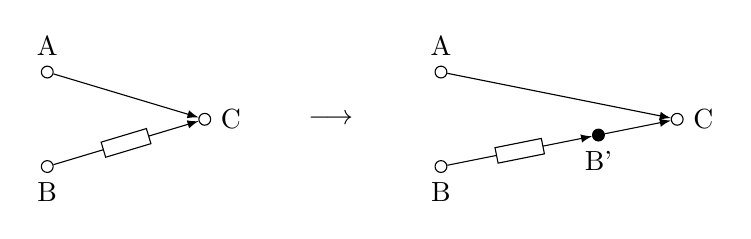
\begin{tikzpicture}[x=2cm, y=1cm]
    \tikzstyle{node0}=[circle, draw, fill=white, inner sep=0pt, minimum size=1.5mm]
    \tikzstyle{node1}=[circle, draw, fill=black, inner sep=0pt, minimum size=1.5mm]

    \node[node0, label=above:A] (A1) at (0, 0) {};
    \node[node0, label=below:B] (B1) at (0, -1.2) {};
    \node[node0, label=right:C] (C1) at (1, -0.6) {};

    \chanSync{A1}{C1}
    \chanFifoOne{B1}{C1}

    \node at (1.8, -0.6) {$\longrightarrow$};

    \node[node0, label=above:A] (A2) at (2.5, 0) {};
    \node[node0, label=below:B] (B2) at (2.5, -1.2) {};
    \node[node1, label=below:B'] (B3) at (3.5, -0.8) {};
    \node[node0, label=right:C] (C2) at (4, -0.6) {};

    \chanSync{A2}{C2}
    \chanFifoOne{B2}{B3}
    \chanSync{B3}{C2}

\end{tikzpicture}
\caption{Adding hidden node to a merger}
    \label{fig:automerger}
\end{figure}

To address this predicament, we develop an automatic merging algorithm \verb|automerger| that enables users to input the nodes only in their original forms without manually adding hidden nodes. The input includes the basic channels and the nodes to be merged. The algorithm will then search for a merger's participant channels, automatically add a hidden node with a unique name to each one (to satisfy the black box checking), and construct a new Sync channel between the hidden node and the merged node. This algorithm simplifies the process of building complex connectors involving mergers and makies the structure more intuitive and user-friendly, avoiding potential errors from manual node addition.

In addition, we upgrade the merger to a multi-merger that can merge more than two input nodes at the same time. The new merger can rearrange the data flows in a chronological order just like the original merger. The implementation of multi-merger can be found at \cite{Z3}. The \verb|automerger| algorithm works well with the multi-merger.

\subsection{Examples of test cases}
We use test cases to validate the correctness of our method, which can be found at \cite{Z3}. Here we choose three representative examples to show how the system works.

\begin{example} % 1. Basic test case
    Fig.\ref{fig:c1} contains four similar connectors, the purpose of which is to output the data flow simultaneously from two sink nodes with a delay. Graph \verb|b|, \verb|c|, and \verb|d| all complete the task perfectly by using a \textit{SyncDrain} channel to synchronize the two flows or just making the delay happens in the same \textit{FIFO1} channel. However, graph \verb|a| fails to achieve the goal since the node B and C are not constrained to be simultanuous. Hence, \verb|b|, \verb|c|, and \verb|d| are equivlent with each other, and are all refinements of \verb|a|.\par
    In our Z3 implementation, we can easily construct these four connectors and check their refinement relations. Graph \verb|a| and \verb|b| can be formalized into
    \begin{verbatim}
c1 = ['Sync A D', 'Sync D E', 'Sync D F', 'Fifo1 E B', 'Fifo1 F C']
c2 = ['Sync A D', 'Sync D E', 'Sync D F', 'Fifo1 E G', 'Fifo1 F H',
      'SyncDrain G H','Sync G B', 'Sync H C']
    \end{verbatim}
    After constructing them into the \verb|Connector| class by the function \verb|automerger|, the result aligns with what we expect: \verb|c1.isRefinementOf(c2, bound)| returns \verb|False| with a counter example, while \verb|c2.isRefinementOf(c1, bound)| returns \verb|True|. The equivalence between \verb|c2|, \verb|c3|, and \verb|c4| can also be verified in the same way.
\end{example}
\begin{figure}[htbp]
    \centering
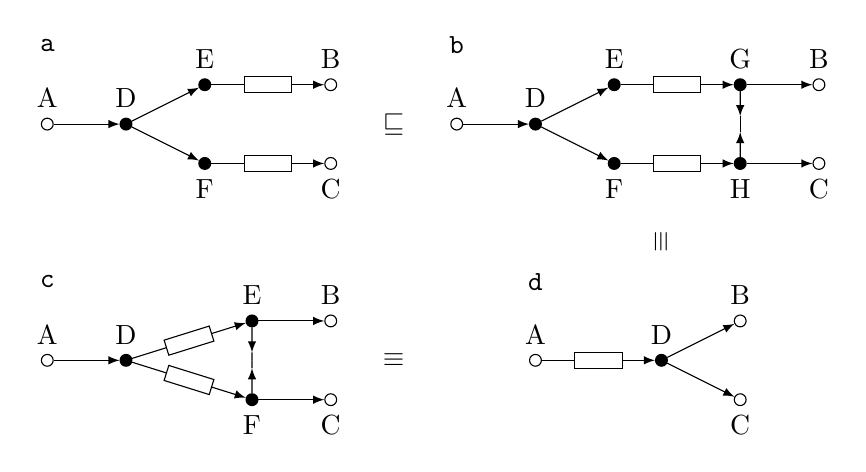
\begin{tikzpicture}[x=2cm, y=1cm]

    % connector 1
    \node[node0, label=above:A] (A1) at (0, -0.5) {};
    \node[node0, label=above:B] (B1) at (1.8, 0) {};
    \node[node0, label=below:C] (C1) at (1.8, -1) {};
    \node[node1, label=above:D] (D1) at (0.5, -0.5) {};
    \node[node1, label=above:E] (E1) at (1, 0) {};
    \node[node1, label=below:F] (F1) at (1, -1) {};

    \chanSync{A1}{D1}
    \chanSync{D1}{E1}
    \chanSync{D1}{F1}
    \chanFifoOne{E1}{B1}
    \chanFifoOne{F1}{C1}

    \node at (0, 0.5) {\verb|a|};

    \node at (2.2, -0.5) {$\sqsubseteq$};

    % connector 2
    \coordinate (off2) at (2.6, 0);
    \node[node0, label=above:A] (A2) at ($(off2) + (0, -0.5)$) {};
    \node[node0, label=above:B] (B2) at ($(off2) + (2.3, 0)$) {};
    \node[node0, label=below:C] (C2) at ($(off2) + (2.3, -1)$) {};
    \node[node1, label=above:D] (D2) at ($(off2) + (0.5, -0.5)$) {};
    \node[node1, label=above:E] (E2) at ($(off2) + (1, 0)$) {};
    \node[node1, label=below:F] (F2) at ($(off2) + (1, -1)$) {};
    \node[node1, label=above:G] (G2) at ($(off2) + (1.8, 0)$) {};
    \node[node1, label=below:H] (H2) at ($(off2) + (1.8, -1)$) {};

    \chanSync{A2}{D2}
    \chanSync{D2}{E2}
    \chanSync{D2}{F2}
    \chanFifoOne{E2}{G2}
    \chanFifoOne{F2}{H2}
    \chanSyncDrain{G2}{H2}
    \chanSync{G2}{B2}
    \chanSync{H2}{C2}

    \node at ($(off2)+(0, 0.5)$) {\verb|b|};

    \node[rotate=90] at (3.9, -2) {$\equiv$};

    % connector 3
    \coordinate (off3) at (0, -3);
    \node[node0, label=above:A] (A1) at ($(off3) + (0, -0.5)$) {};
    \node[node0, label=above:B] (B1) at ($(off3) + (1.8, 0)$) {};
    \node[node0, label=below:C] (C1) at ($(off3) + (1.8, -1)$) {};
    \node[node1, label=above:D] (D1) at ($(off3) + (0.5, -0.5)$) {};
    \node[node1, label=above:E] (E1) at ($(off3) + (1.3, 0)$) {};
    \node[node1, label=below:F] (F1) at ($(off3) + (1.3, -1)$) {};

    \chanSync{A1}{D1}
    \chanFifoOne{D1}{E1}
    \chanFifoOne{D1}{F1}
    \chanSyncDrain{E1}{F1}
    \chanSync{E1}{B1}
    \chanSync{F1}{C1}

    \node at ($(off3)+(0, 0.5)$) {\verb|c|};

    \node at (2.2, -3.5) {$\equiv$};

    % connector 4
    \coordinate (off4) at (3.1, -3);
    \node[node0, label=above:A] (A1) at ($(off4) + (0, -0.5)$) {};
    \node[node0, label=above:B] (B1) at ($(off4) + (1.3, 0)$) {};
    \node[node0, label=below:C] (C1) at ($(off4) + (1.3, -1)$) {};
    \node[node1, label=above:D] (D1) at ($(off4) + (0.8, -0.5)$) {};

    \chanFifoOne{A1}{D1}
    \chanSync{D1}{B1}
    \chanSync{D1}{C1}

    \node at ($(off4)+(0, 0.5)$) {\verb|d|};

\end{tikzpicture}
\caption{Basic test case}
    \label{fig:c1}
\end{figure}

\begin{example} % 2. Time-based test case
    The left graph in Fig.\ref{fig:c2} is called Lower Bounded FIFO1, which aims to output the data flow with a delay of at least $t$ time units. The right graph is a mutated connector of the former one, since it requires the output time to be exactly $t$ time units later than the input time. Hence in Z3 implementation, the result of \verb|isRefinementOf| between the two connectors would be both \verb|False| with counter examples.
\end{example}
\begin{figure}[htbp]
    \centering
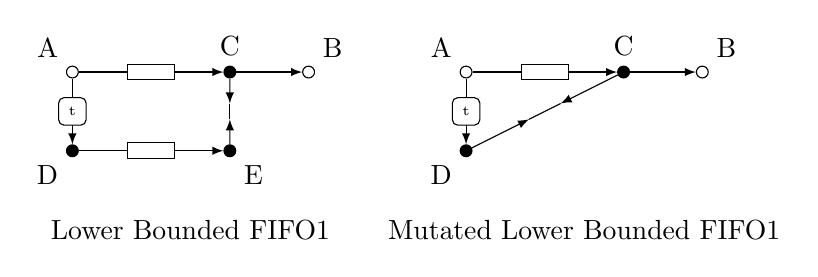
\begin{tikzpicture}[x=2cm, y=1cm]

    % connector 1
    \node[node0, label=above left:A] (A1) at (0, 0) {};
    \node[node0, label=above right:B] (B1) at (1.5, 0) {};
    \node[node1, label=above:C] (C1) at (1, 0) {};
    \node[node1, label=below left:D] (D1) at (0, -1) {};
    \node[node1, label=below right:E] (E1) at (1, -1) {};

    \chanFifoOne{A1}{C1}
    \chanTimert{A1}{D1}{t}
    \chanFifoOne{D1}{E1}
    \chanSyncDrain{C1}{E1}
    \chanSync{C1}{B1}

    \node at (0.75, -2) {Lower Bounded FIFO1};

    % connector 2
    \coordinate (off) at (2.5, 0);
    \node[node0, label=above left:A] (A2) at ($(off) + (0, 0)$) {};
    \node[node0, label=above right:B] (B2) at ($(off) + (1.5, 0)$) {};
    \node[node1, label=above:C] (C2) at ($(off) + (1, 0)$) {};
    \node[node1, label=below left:D] (D2) at ($(off) + (0, -1)$) {};

    \chanFifoOne{A2}{C2}
    \chanTimert{A2}{D2}{t}
    \chanSyncDrain{C2}{D2}
    \chanSync{C2}{B2}

    \node at ($(off)+(0.75, -2)$) {Mutated Lower Bounded FIFO1};

\end{tikzpicture}
\caption{Time-based test case}
    \label{fig:c2}
\end{figure}

\begin{example} % 3. Probability-based test case
    In the third example, we combine a timer channel and a probabilistic channel to form a complex connector and its mutation as shown in Fig.\ref{fig:c3}. The two connectors are supposed to output a random signal between 0 and 1 after a delay of $t$ time units. The two connectors only differ where the random signal is generated: before or after the delay. Therefore, they are equivalent, i.e., a refinement of each other. In Z3 implementation, we can verify this quivalence by verifying the \verb|True| output of the \verb|isRefinementOf| function in both directions.
\end{example}
\begin{figure}[htbp]
    \centering
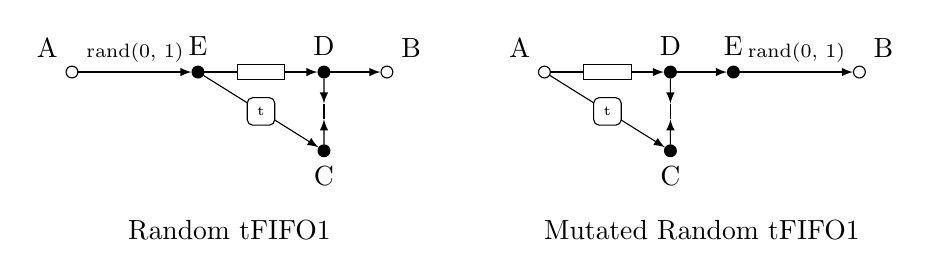
\begin{tikzpicture}[x=2cm, y=1cm]

    % connector 1
    \node[node0, label=above left:A] (A1) at (0, 0) {};
    \node[node0, label=above right:B] (B1) at (2, 0) {};
    \node[node1, label=below:C] (C1) at (1.6, -1) {};
    \node[node1, label=above:D] (D1) at (1.6, 0) {};
    \node[node1, label=above:E] (E1) at (0.8, 0) {};

    \chanRdmSync{A1}{E1}{rand(0, 1)}
    \chanFifoOne{E1}{D1}
    \chanTimert{E1}{C1}{t}
    \chanSyncDrain{C1}{D1}
    \chanSync{D1}{B1}

    \node at (1, -2) {Random tFIFO1};

    % connector 2
    \coordinate (off) at (3, 0);
    \node[node0, label=above left:A] (A1) at ($(off) + (0, 0)$) {};
    \node[node0, label=above right:B] (B1) at ($(off) + (2, 0)$) {};
    \node[node1, label=below:C] (C1) at ($(off) + (0.8, -1)$) {};
    \node[node1, label=above:D] (D1) at ($(off) + (0.8, 0)$) {};
    \node[node1, label=above:E] (E1) at ($(off) + (1.2, 0)$) {};

    \chanSync{D1}{E1}
    \chanFifoOne{A1}{D1}
    \chanTimert{A1}{C1}{t}
    \chanSyncDrain{C1}{D1}
    \chanRdmSync{E1}{B1}{rand(0, 1)}

    \node at ($(off)+(1, -2)$) {Mutated Random tFIFO1};

\end{tikzpicture}
\caption{Probability-based test case}
    \label{fig:c3}
\end{figure}





\nocite{*}
\bibliography{reference}

\end{document}
